\documentclass[11pt]{article}
\usepackage[utf8]{inputenc}
\usepackage[T1]{fontenc}
\usepackage{amsmath}
\usepackage{amssymb}
\usepackage{multicol}
\usepackage{geometry}
\usepackage{tikz}
\usepackage{enumitem}
\usepackage{xcolor}
\usepackage{titlesec}

% Configurações de layout
\geometry{a4paper, left=1cm, right=1cm, top=0.5cm, bottom=1.2cm}
\setlength{\columnseprule}{0.4pt}

% Cores para títulos
\titleformat{\section}{\normalfont\Large\bfseries\color{blue}}{\thesection}{1em}{}
\titleformat{\subsection}{\normalfont\large\bfseries\color{red}}{\thesubsection}{1em}{}

% Reduz espaço antes e depois de seções e subseções
\titlespacing{\section}{0pt}{2ex}{1ex}
\titlespacing{\subsection}{0pt}{1.5ex}{0.5ex}

% Reduz espaço entre paragrafos 
\setlength{\parskip}{0pt}
\setlength{\parindent}{0pt}

% Comandos personalizados
\newcommand{\respostaNum}[1]{\textcolor{blue}{\boxed{#1}}}
\newcommand{\respostaTxt}[1]{\textcolor{blue}{#1}}
\newcommand{\resolucao}{\textbf{\textcolor{blue}{Resolução:}}}
\newcommand{\etapa}[1]{\textbf{\textcolor{red}{Etapa #1:}}}

\title{\textcolor{red}{Gabarito Comentado: Porcentagem (\%)}}
\author{Professor: Jefferson}
\date{}

\begin{document}

\maketitle
\vspace{-1cm}

\begin{multicols}{2}

\section*{Instruções}
\textbf{Verifique suas respostas e estude as resoluções comentadas.}

\section*{Gabarito - Exercícios Básicos}

\begin{enumerate}[leftmargin=*]

\item \textbf{Converta para forma decimal:}

\begin{enumerate}[label=\alph*)]
\item 15\%

\resolucao
\[
15\% = \frac{15}{100} = \respostaNum{0,15}
\]

\item 8\%

\resolucao
\[
8\% = \frac{8}{100} = \respostaNum{0,08}
\]

\item 120\%

\resolucao
\[
120\% = \frac{120}{100} = \respostaNum{1,2}
\]

\item 0,5\%

\resolucao
\[
0,5\% = \frac{0,5}{100} = \respostaNum{0,005}
\]
\end{enumerate}

\item \textbf{Converta para porcentagem:}

\begin{enumerate}[label=\alph*)]
\item 0,25

\resolucao
\[
0,25 = \frac{25}{100} = \respostaNum{25\%}
\]

\item 0,75

\resolucao
\[
0,75 = \frac{75}{100} = \respostaNum{75\%}
\]

\item 1,5

\resolucao
\[
1,5 = \frac{150}{100} = \respostaNum{150\%}
\]

\item 0,02

\resolucao
\[
0,02 = \frac{2}{100} = \respostaNum{2\%}
\]
\end{enumerate}

\item \textbf{Calcule:}

\begin{enumerate}[label=\alph*)]
\item 30\% de 200

\resolucao

\textbf{\textcolor{red}{Etapa 1:}} Transformar 30\% em decimal: $30\% = 0,30$

\textbf{\textcolor{red}{Etapa 2:}} Multiplicar: $0,30 \times 200 = \respostaNum{60}$

\item 12\% de 500

\resolucao

$0,12 \times 500 = \respostaNum{60}$

\item 25\% de 80

\resolucao

$0,25 \times 80 = \respostaNum{20}$

\item 8\% de 150

\resolucao

$0,08 \times 150 = \respostaNum{12}$
\end{enumerate}

\item \textbf{Complete a tabela:}

\begin{center}
\begin{tabular}{|c|c|c|}
\hline
\textbf{Total} & \textbf{Porcentagem} & \textbf{Valor} \\
\hline
300 & 20\% & \textcolor{blue}{60} \\
500 & 15\% & \textcolor{blue}{75} \\
200 & \textcolor{blue}{25\%} & 50 \\
400 & \textcolor{blue}{8\%} & 32 \\
\hline
\end{tabular}
\end{center}

\resolucao

\textbf{1ª linha:} $0,20 \times 300 = 60$

\textbf{2ª linha:} $0,15 \times 500 = 75$

\textbf{3ª linha:} $\frac{50}{200} \times 100\% = 0,25 \times 100\% = 25\%$

\textbf{4ª linha:} $\frac{32}{400} \times 100\% = 0,08 \times 100\% = 8\%$

\item \textbf{Problemas de desconto:}

\begin{enumerate}[label=\alph*)]
\item Calça: R\$ 120,00 com 20\% de desconto

\resolucao

\textbf{\textcolor{red}{Etapa 1:}} Calcular o desconto: $0,20 \times 120 = 24$

\textbf{\textcolor{red}{Etapa 2:}} Subtrair: $120 - 24 = \respostaNum{R\$ 96,00}$

\textbf{OU fórmula direta:} $120 \times (1 - 0,20) = 120 \times 0,80 = 96$

\item Celular: R\$ 800,00 com 12\% de desconto

\resolucao

$800 \times (1 - 0,12) = 800 \times 0,88 = \respostaNum{R\$ 704,00}$
\end{enumerate}

\item \textbf{Problemas de aumento:}

\begin{enumerate}[label=\alph*)]
\item Aluguel: R\$ 600,00 com aumento de 8\%

\resolucao

\textbf{\textcolor{red}{Etapa 1:}} Calcular o aumento: $0,08 \times 600 = 48$

\textbf{\textcolor{red}{Etapa 2:}} Somar: $600 + 48 = \respostaNum{R\$ 648,00}$

\textbf{OU fórmula direta:} $600 \times (1 + 0,08) = 600 \times 1,08 = 648$

\item Salário: R\$ 1500,00 com aumento de 5\%

\resolucao

$1500 \times 1,05 = \respostaNum{R\$ 1575,00}$
\end{enumerate}

\item \textbf{Calcule a taxa percentual:}

\begin{enumerate}[label=\alph*)]
\item 30 acertos em 40 questões

\resolucao

\textbf{\textcolor{red}{Etapa 1:}} Dividir parte pelo todo: $\frac{30}{40} = 0,75$

\textbf{\textcolor{red}{Etapa 2:}} Multiplicar por 100\%: $0,75 \times 100\% = \respostaNum{75\%}$

\item 12 meninas em 30 alunos

\resolucao

$\frac{12}{30} = 0,4 \times 100\% = \respostaNum{40\%}$

\item 45 gols em 60 jogos

\resolucao

$\frac{45}{60} = 0,75 \times 100\% = \respostaNum{75\%}$

\item R\$ 18,00 de desconto em R\$ 120,00

\resolucao

$\frac{18}{120} = 0,15 \times 100\% = \respostaNum{15\%}$
\end{enumerate}

\item \textbf{Problemas com porcentagem:}

\begin{enumerate}[label=\alph*)]
\item Prova de 50 questões, acertei 40

\resolucao

$\frac{40}{50} = 0,8 \times 100\% = \respostaNum{80\%}$

\item Loja vendeu 180 de 200 produtos

\resolucao

$\frac{180}{200} = 0,9 \times 100\% = \respostaNum{90\%}$

\item 500 alunos, 125 usam óculos

\resolucao

$\frac{125}{500} = 0,25 \times 100\% = \respostaNum{25\%}$
\end{enumerate}
\end{enumerate}

\section*{Gabarito - Exercícios Intermediários}

\begin{enumerate}[leftmargin=*, start=9]

\item \textbf{Aumentos e descontos sucessivos:}

\begin{enumerate}[label=\alph*)]
\item Dois aumentos sucessivos de 10\%

\resolucao

\textbf{\textcolor{red}{Etapa 1:}} Fator para 10\%: $1 + 0,10 = 1,10$

\textbf{\textcolor{red}{Etapa 2:}} Multiplicar: $1,10 \times 1,10 = 1,21$

\textbf{\textcolor{red}{Etapa 3:}} Taxa total: $(1,21 - 1) \times 100\% = \respostaNum{21\%}$

\item Desconto de 20\% e depois 10\%

\resolucao

\textbf{\textcolor{red}{Etapa 1:}} Fator para 20\%: $1 - 0,20 = 0,80$

\textbf{\textcolor{red}{Etapa 2:}} Fator para 10\%: $1 - 0,10 = 0,90$

\textbf{\textcolor{red}{Etapa 3:}} Multiplicar: $0,80 \times 0,90 = 0,72$

\textbf{\textcolor{red}{Etapa 4:}} Desconto total: $(1 - 0,72) \times 100\% = \respostaNum{28\%}$
\end{enumerate}

\item \textbf{Calcule o valor original:}

\begin{enumerate}[label=\alph*)]
\item Após aumento de 15\% passou a R\$ 230,00

\resolucao

\textbf{\textcolor{red}{Etapa 1:}} Fator de aumento: $1 + 0,15 = 1,15$

\textbf{\textcolor{red}{Etapa 2:}} Valor original = $\frac{230}{1,15} = \respostaNum{R\$ 200,00}$

\item Com desconto de 25\% paguei R\$ 150,00

\resolucao

\textbf{\textcolor{red}{Etapa 1:}} Fator de desconto: $1 - 0,25 = 0,75$

\textbf{\textcolor{red}{Etapa 2:}} Valor original = $\frac{150}{0,75} = \respostaNum{R\$ 200,00}$
\end{enumerate}

\item \textbf{Comparação percentual:}

\begin{enumerate}[label=\alph*)]
\item João R\$ 200, Pedro R\$ 150. Quanto João tem a mais?

\resolucao

\textbf{\textcolor{red}{Etapa 1:}} Diferença: $200 - 150 = 50$

\textbf{\textcolor{red}{Etapa 2:}} Porcentagem em relação a Pedro: $\frac{50}{150} \times 100\% \approx \respostaNum{33,33\%}$

\item 15 gostam de Matemática, 25 de Português

\resolucao

\textbf{\textcolor{red}{Etapa 1:}} Diferença: $25 - 15 = 10$

\textbf{\textcolor{red}{Etapa 2:}} Porcentagem em relação a Matemática: $\frac{10}{15} \times 100\% \approx \respostaNum{66,67\%}$
\end{enumerate}

\item \textbf{Situações do dia a dia:}

\begin{enumerate}[label=\alph*)]
\item Investimento de R\$ 1000,00 rendeu 12\%

\resolucao

$1000 \times 1,12 = \respostaNum{R\$ 1120,00}$

\item População de 5000 cresceu 8\%

\resolucao

$5000 \times 1,08 = \respostaNum{5400 \text{ habitantes}}$

\item Carro de R\$ 40.000,00 desvalorizou 15\%

\resolucao

$40000 \times 0,85 = \respostaNum{R\$ 34.000,00}$
\end{enumerate}

\item \textbf{Interpretação de gráfico (pizza):}

\begin{center}
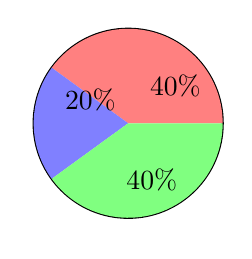
\begin{tikzpicture}[scale=0.6]
\draw[thick] (0,0) circle (2cm);
\fill[red!50] (0,0) -- (0:2cm) arc (0:144:2cm) -- cycle;
\fill[blue!50] (0,0) -- (144:2cm) arc (144:216:2cm) -- cycle;
\fill[green!50] (0,0) -- (216:2cm) arc (216:360:2cm) -- cycle;
\node at (1,0.8) {40\%};
\node at (-0.8,0.5) {20\%};
\node at (0.5,-1.2) {40\%};
\end{tikzpicture}
\end{center}

Total de pessoas: 500

\resolucao

\textbf{\textcolor{red}{Etapa 1:}} Setor vermelho (40\%): $0,40 \times 500 = \respostaNum{200}$

\textbf{\textcolor{red}{Etapa 2:}} Setor azul (20\%): $0,20 \times 500 = \respostaNum{100}$

\textbf{\textcolor{red}{Etapa 3:}} Setor verde (40\%): $0,40 \times 500 = \respostaNum{200}$

\item \textbf{Porcentagem de porcentagem:}

\begin{enumerate}[label=\alph*)]
\item 20\% de 30\% de 500

\resolucao

\textbf{\textcolor{red}{Etapa 1:}} 30\% de 500: $0,30 \times 500 = 150$

\textbf{\textcolor{red}{Etapa 2:}} 20\% de 150: $0,20 \times 150 = \respostaNum{30}$

\item 50\% de 10\% de 1000

\resolucao

\textbf{\textcolor{red}{Etapa 1:}} 10\% de 1000: $0,10 \times 1000 = 100$

\textbf{\textcolor{red}{Etapa 2:}} 50\% de 100: $0,50 \times 100 = \respostaNum{50}$
\end{enumerate}
\end{enumerate}

\section*{Gabarito - Exercícios Avançados}

\begin{enumerate}[leftmargin=*, start=15]

\item \textbf{Dois aumentos sucessivos: 10\% e 15\%}

\resolucao

\textbf{\textcolor{red}{Etapa 1:}} Fator 1: $1,10$

\textbf{\textcolor{red}{Etapa 2:}} Fator 2: $1,15$

\textbf{\textcolor{red}{Etapa 3:}} Fator total: $1,10 \times 1,15 = 1,265$

\textbf{\textcolor{red}{Etapa 4:}} Aumento total: $(1,265 - 1) \times 100\% = \respostaNum{26,5\%}$

\item \textbf{Descontos sucessivos: 10\% e 5\%}

\resolucao

\textbf{\textcolor{red}{Etapa 1:}} Fator 1: $0,90$

\textbf{\textcolor{red}{Etapa 2:}} Fator 2: $0,95$

\textbf{\textcolor{red}{Etapa 3:}} Fator total: $0,90 \times 0,95 = 0,855$

\textbf{\textcolor{red}{Etapa 4:}} Desconto único: $(1 - 0,855) \times 100\% = \respostaNum{14,5\%}$

\item \textbf{60\% são mulheres, 25\% das mulheres usam óculos}

\resolucao

\textbf{\textcolor{red}{Etapa 1:}} Mulheres: $60\%$ do total

\textbf{\textcolor{red}{Etapa 2:}} Mulheres de óculos: $25\%$ das mulheres

\textbf{\textcolor{red}{Etapa 3:}} $0,25 \times 0,60 = 0,15 = \respostaNum{15\%}$ do total

\item \textbf{Mercadoria: R\$ 200,00 +20\% -20\%}

\resolucao

\textbf{\textcolor{red}{Etapa 1:}} Após aumento: $200 \times 1,20 = 240$

\textbf{\textcolor{red}{Etapa 2:}} Após desconto: $240 \times 0,80 = \respostaNum{R\$ 192,00}$

\textbf{Observação:} O preço final é menor que o original!

\item \textbf{Pesquisa: 40\% produto A, 35\% produto B, resto C. 50 pessoas preferem C.}

\resolucao

\textbf{\textcolor{red}{Etapa 1:}} Porcentagem de C: $100\% - 40\% - 35\% = 25\%$

\textbf{\textcolor{red}{Etapa 2:}} 25\% corresponde a 50 pessoas

\textbf{\textcolor{red}{Etapa 3:}} Total: $\frac{50}{0,25} = \respostaNum{200 \text{ pessoas}}$

\item \textbf{Salário R\$ 2000,00 +8\% +5\%}

\resolucao

\textbf{\textcolor{red}{Etapa 1:}} Após 8\%: $2000 \times 1,08 = 2160$

\textbf{\textcolor{red}{Etapa 2:}} Após 5\%: $2160 \times 1,05 = \respostaNum{R\$ 2268,00}$

\textbf{OU:} $2000 \times 1,08 \times 1,05 = 2000 \times 1,134 = 2268$

\item \textbf{Calcule o valor inicial:}

\begin{enumerate}[label=\alph*)]
\item Dois aumentos de 10\%, valor final R\$ 484,00

\resolucao

\textbf{\textcolor{red}{Etapa 1:}} Fator total: $1,10 \times 1,10 = 1,21$

\textbf{\textcolor{red}{Etapa 2:}} Valor inicial: $\frac{484}{1,21} = \respostaNum{R\$ 400,00}$

\item Dois descontos de 20\%, valor final R\$ 320,00

\resolucao

\textbf{\textcolor{red}{Etapa 1:}} Fator total: $0,80 \times 0,80 = 0,64$

\textbf{\textcolor{red}{Etapa 2:}} Valor inicial: $\frac{320}{0,64} = \respostaNum{R\$ 500,00}$
\end{enumerate}

\item \textbf{Gráfico de sorvete: 200 pessoas}

\begin{center}
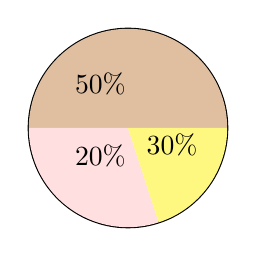
\begin{tikzpicture}[scale=0.7]
\draw[thick] (0,0) circle (1.8cm);
\fill[brown!50] (0,0) -- (0:1.8cm) arc (0:180:1.8cm) -- cycle;
\fill[pink!50] (0,0) -- (180:1.8cm) arc (180:288:1.8cm) -- cycle;
\fill[yellow!50] (0,0) -- (288:1.8cm) arc (288:360:1.8cm) -- cycle;
\node at (-0.5,0.8) {50\%};
\node at (0.8,-0.3) {30\%};
\node at (-0.5,-0.5) {20\%};
\end{tikzpicture}
\end{center}

\resolucao

\textbf{\textcolor{red}{Etapa 1:}} Chocolate (50\%): $0,50 \times 200 = \respostaNum{100}$

\textbf{\textcolor{red}{Etapa 2:}} Morango (30\%): $0,30 \times 200 = \respostaNum{60}$

\textbf{\textcolor{red}{Etapa 3:}} Baunilha (20\%): $0,20 \times 200 = \respostaNum{40}$
\end{enumerate}

\section*{Resumo das Fórmulas}

\begin{center}
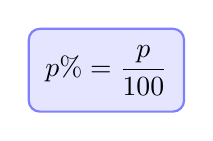
\begin{tikzpicture}
\node[rectangle, fill=blue!10, rounded corners, inner sep=6pt, draw=blue!50, thick] (box) {
$\displaystyle p\% = \frac{p}{100}$
};
\end{tikzpicture}

\vspace{0.2cm}

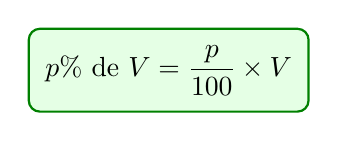
\begin{tikzpicture}
\node[rectangle, fill=green!10, rounded corners, inner sep=6pt, draw=green!50!black, thick] (box) {
$\displaystyle p\% \text{ de } V = \frac{p}{100} \times V$
};
\end{tikzpicture}

\vspace{0.2cm}

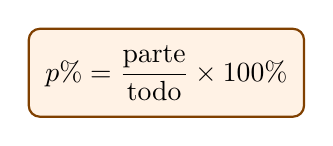
\begin{tikzpicture}
\node[rectangle, fill=orange!10, rounded corners, inner sep=6pt, draw=orange!50!black, thick] (box) {
$\displaystyle p\% = \frac{\text{parte}}{\text{todo}} \times 100\%$
};
\end{tikzpicture}

\vspace{0.2cm}

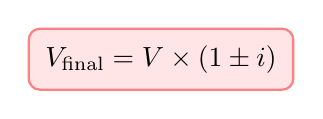
\begin{tikzpicture}
\node[rectangle, fill=red!10, rounded corners, inner sep=6pt, draw=red!50, thick] (box) {
$\displaystyle V_{\text{final}} = V \times (1 \pm i)$
};
\end{tikzpicture}
\end{center}

\vspace{0.3cm}
\textcolor{blue}{\textbf{Legenda:}} 
\begin{itemize}
\item \textcolor{blue}{Respostas numéricas:} \respostaNum{exemplo}
\item \textcolor{blue}{Respostas textuais:} \textcolor{blue}{exemplo}
\end{itemize}

\vspace{0.3cm}
\textcolor{red}{\textbf{Fatores importantes:}}
\begin{itemize}
\item \textcolor{blue}{Aumento:} $(1 + i)$
\item \textcolor{blue}{Desconto:} $(1 - i)$
\item \textcolor{blue}{Aumentos sucessivos:} $(1 + i_1) \times (1 + i_2)$
\item \textcolor{blue}{Descontos sucessivos:} $(1 - i_1) \times (1 - i_2)$
\end{itemize}

\end{multicols}

\end{document}
